\documentclass{article}

\usepackage{tikz}
\usepackage{pgfplots}
\pgfplotsset{compat=1.17} 
\begin{document}
	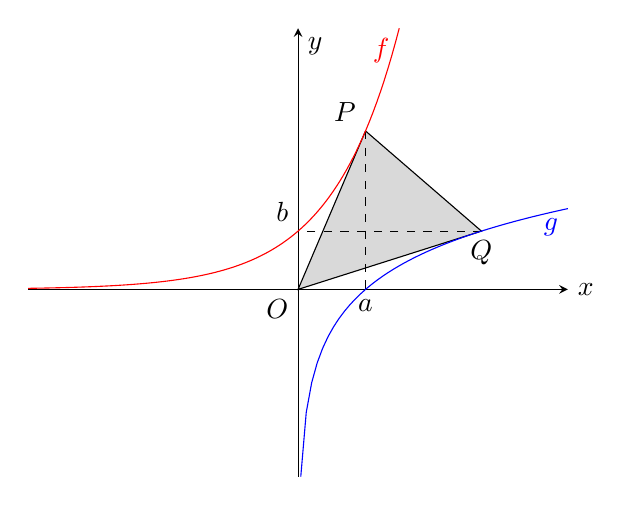
\begin{tikzpicture}
		\begin{axis}
			[
				axis lines = center, 
				ticks = none,
				every axis x label/.style={at={(current axis.right of origin)},anchor=west},
				xlabel=$x$,
				ylabel=$y$
			]
			\draw[fill=gray!30] (0,0) -- (1,e^1) -- (e^1, 1) -- cycle;
			\draw[thin, dashed] (1,e^1) -- (1,0) node[below] {\(a\)};
			\draw[thin, dashed] (e^1,1) -- (0,1) node[above left] {\(b\)};
			\addplot [domain=-4:4, samples=100, color=blue] {ln(x)} node[below left]{\(g\)};
			\addplot [domain=-4:1.5, samples=100, color=red] {e^x} node[below left] {\(f\)};
			\node at (0,0) [below left] {\(O\)};
			\node at (1,e^1) [above left] {\(P\)};
			\node at (e^1,1) [below] {\(Q\)};
		\end{axis}
	\end{tikzpicture}
\end{document}
